\documentclass[11pt,a4paper]{article}

% Note: Must use TexLive 2016 and NOT 2018 or later.
% See notes here: https://www.overleaf.com/latex/templates/acl-2020-proceedings-template/zsrkcwjptpcd

\usepackage[T1]{fontenc} 
\usepackage[utf8]{inputenc}
\usepackage[english]{babel}

\usepackage[hyperref]{acl2020}
\usepackage[all]{hypcap}
\usepackage{times}
\usepackage{latexsym}
\renewcommand{\UrlFont}{\ttfamily\small}

% This is not strictly necessary, and may be commented out,
% but it will improve the layout of the manuscript,
% and will typically save some space.
\usepackage{microtype}

\usepackage{todonotes}
\usepackage{csquotes}
\usepackage{caption}
\usepackage{hyperref}
\usepackage{subcaption}
\usepackage{multirow}
\usepackage{booktabs}
\usepackage{orcidlink}

\aclfinalcopy % Uncomment this line for the final submission

% \setlength\titlebox{5cm}
% You can expand the titlebox if you need extra space
% to show all the authors. Please do not make the titlebox
% smaller than 5cm (the original size); we will check this
% in the camera-ready version and ask you to change it back.

\newcommand\BibTeX{B\textsc{ib}\TeX}

\title{Speech2Text in JoeyNMT}

\author{\small Stefan Machmeier\,\orcidlink{0000-0002-7028-1755} \\
  \small Department of Computer Science \\
  \small Heidelberg University, Germany \\
  \small \textit{tz251@stud.uni-heidelberg.de} \\
  \And
  \small Robin Fleige \\
  \small Department of Computer Science \\
  \small Heidelberg University, Germany \\
  \small \textit{lq250@stud.uni-heidelberg.de} \\
  \And
  \small Andre Meyering\,\orcidlink{0000-0002-7973-0369} \\
  \small Department of Computer Science \\
  \small Heidelberg University, Germany \\
  \small \textit{hp250@stud.uni-heidelberg.de} \\}

\date{\today}

\begin{document}
\maketitle
\begin{abstract}
In this paper we are looking into speech to text transformations using the JoeyNMT neural machine translation toolkit.
We adapt JoeyNMT's existing code base to additionally handle audio files that are then translated to text.
We achieve this by including Torchaudio, the audio counterpart of the Torchtext project which is heavily used by JoeyNMT.
Even a small dataset shows promising results.
\end{abstract}

\section{Introduction}
In this paper an approach to use JoeyNMT for processing speech to text is worked out.
Instead of translating text to text, we translate speech to text.
For this purpose, the Mel Frequency Cepstral Coefficients (MFCC) of the audio files is used as input for JoeyNMT.
As dataset we use audio files from the Common Voice project for the German language.

\section{Related Work}

Speech to text transformations are common but in context of JoeyNMT, we found that it references only one project that works with audio files.
\enquote{Speech Joey}~\cite{speechjoey} extends JoeyNMT with functionality for speech recognition and is written by Sariya Karimova\footnote{See \url{https://www.cl.uni-heidelberg.de/~karimova/}, last visited on 2021-09-09}, a former graduate research assistant at the Statistical NLP group of the Heidelberg University.
However, the project does not run anymore due to breaking changes in the project's
dependencies and missing explicit version numbers in their list of dependencies.
Furthermore, after trying to install older versions of certain dependencies,
we noticed that some were not available for more recent versions of Python such as 3.8 or 3.9.
We still looked at the project as it was listed by JoeyNMT itself.
In comparison to our project\footnote{See \url{https://github.com/bugwelle/cl-neural-networks}, last visited on 2021-09-10}, Speech Joey uses \enquote{librosa}\footnote{See \url{https://librosa.org/doc/latest/index.html}, last visited on 2021-09-10}, whereas we use Torchaudio\footnote{See \url{https://github.com/pytorch/audio}, last visited on 2021-09-10}.
The underlying transformations should still be very similar but we were unable to compare our results against Speech Joey due to the issues mentioned earlier.


\section{JoeyNMT}
JoeyNMT is an open source project for neural machine
translation~(NMT) that aims to be easy to understand while implementing modern approaches.
This gives beginners the possibility to quickly and easily understand the architecture and customize individual parts to experiment with the behavior.
Since JoeyNMT's goal is to be as simple to understand as possible, they are guided by the 80/20 approach, which in this case means they want to enable 80\% of the functionality with 20\% of the code.
JoeyNMT implements a Recurrent Neural Network~(RNN) encoder-decoder using Gated Recurrent Unit~(GRU) or Long Short Term Memory~(LSTM) units.
It also provides the possibility to use either a multi-layer perceptron or a bilinear interpolation as attention function.
Also JoeyNMT supports word based, character based and also Byte Pair Encoding~(BPE) based encodings.
In the configuration file that JoeyNMT provides, you can adjust the hyperparameters of the Neural Network. 
\cite{DBLP:journals/corr/abs-1907-12484}

\section{Speech To Text}

Speech to Text is a process that converts speech in audio form to text. 
This is used in many different areas today, for example in the generation of subtitles for accessibility or for digital assistants such as Alexa, Siri, Cortana or Google Home.

\subsection{Feature Extraction}

As audio files are just binary blobs and cannot be worked with as text,
we cannot work with JoeyNMT's existing feature extractions for text.

For audio processing, there are multiple common ways to represent audio signals in a way that features can be easily extracted.
One common way is the waveform representation as can be seen in \autoref{fig:1021_waveform} on \autopageref{fig:1021_waveform} for one of our training audio files.
The figure visualizes amplitude changes over time.
Its benefit lies in the audio detection, where values near zero indicate silence
and larger amplitudes indicate louder sounds.
It can not only be used to detect pauses between spoken words, but it is also possible to detect voiced and unvoiced sounds and even certain vowels can be detected~\cite{Comer_1162014}.

Another way to visualize audio signals are Spectrograms, as can be seen in \autoref{fig:1021_spectrogramm}.
The waveform is visualized as a Spectrogram and shows more details of the audio signals, or rather, it shows the spectrum of frequencies over time.
Oftentimes, the Mel frequency spectrum is used~\cite{MelFreq} as this represents the human audio perception.

However, there are further frequency transformations of audio signals
that can be used to better extract features to translate spoken to written words.

According to Wang and Lawlor, \enquote{MFCC is one of more the successful methods} for speech to text systems which is \enquote{based on the human peripheral auditory system}~\cite{Wang_7983644}.
Therefore, MFCC (short for Mel Frequency Cepstral Coefficients) is another transformation that yields good results for speech recognition.
\autoref{fig:1021_mfcc} shows the resulting spectrogram after applying MFCC.
We note that there are possibilities to improve results even more, as described in \cite{Winursito_8350748}.

We refer to \cite{ittichaichareon2012speech} and \cite{singh2014approach} for a detailed description of MFCC.
 
\begin{figure*}[htb]
    \begin{subfigure}[b]{0.32\textwidth}
        \centering
        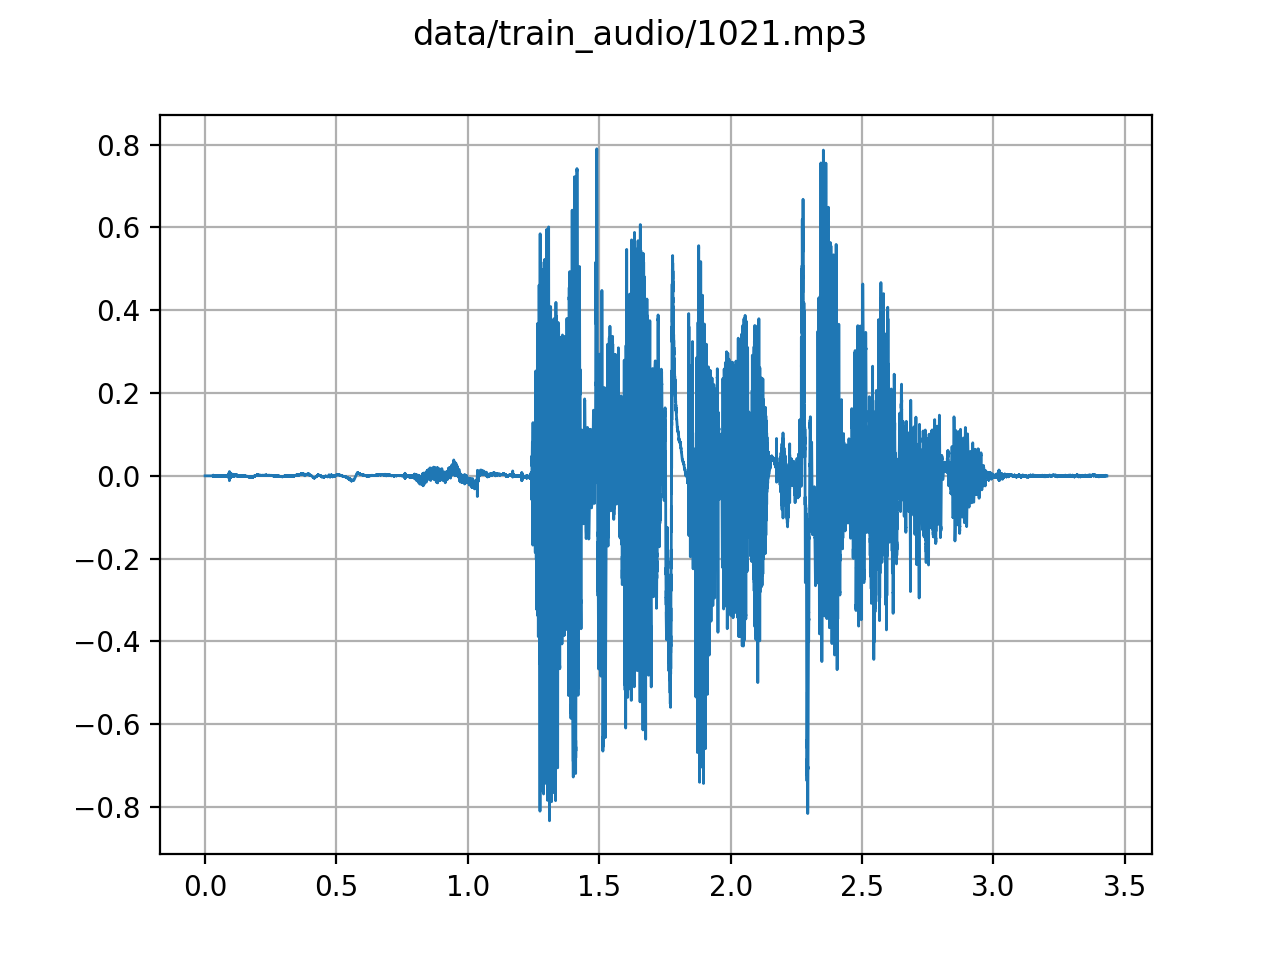
\includegraphics[width=\textwidth]{joeynmt-speech2text/images/1021_Eine_Beleuchtung_ist_vorgeschrieben_Waveform.png}
        \caption{Waveform}
        \label{fig:1021_waveform}
    \end{subfigure}
     \hfill
    \begin{subfigure}[b]{0.32\textwidth}
        \centering
        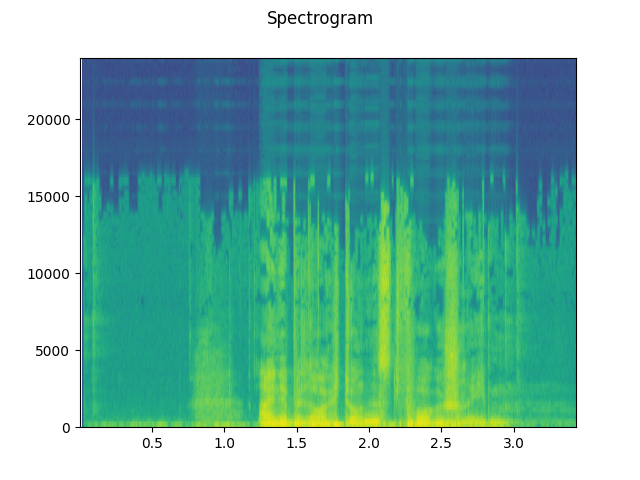
\includegraphics[width=\textwidth]{joeynmt-speech2text/images/1021_Eine_Beleuchtung_ist_vorgeschrieben_Spectrogram.png}
        \caption{Spectrogramm}
        \label{fig:1021_spectrogramm}
    \end{subfigure}
     \hfill
    \begin{subfigure}[b]{0.32\textwidth}
        \centering
        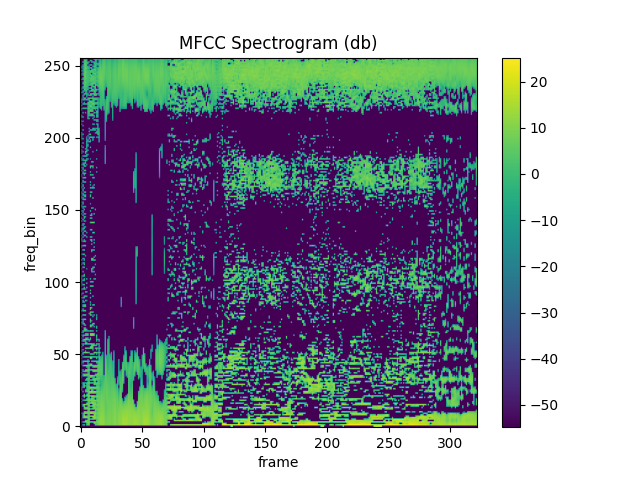
\includegraphics[width=\textwidth]{joeynmt-speech2text/images/1021_Eine_Beleuchtung_ist_vorgeschrieben_MFCC.png}
        \caption{MFCC}
        \label{fig:1021_mfcc}
    \end{subfigure}
    \caption{Visualizations of \enquote{Eine Beleuchtung ist vorgeschrieben.}}
    \label{fig:beleuchtung_viz}
\end{figure*}

\subsection{Dataset}
\label{subsec:dataset}

The dataset used throughout this paper is the open \enquote{Common Voice Corpus 7.0} dataset by Mozilla~\cite{commonvoice:2020}.
We have chosen the German language as that's what the authors are most familiar with, which allows us to better evaluate the dataset quality.
The unprocessed dataset contains 26\,GB of audio files which 1035 hours of spoken text according to \enquote{Common Voice}.

After listening to few audio files, the authors decided to filter the dataset for one major reason:
There were audio files that had accents that made it hard to understand even for native speakers.

Furthermore, even though the authors think that enterprise speech to text models
should handle accents as well as differences between male and female voices,
we decided that it would be out-of-scope for this paper.
Therefore, all audio files were filtered according to these rules:

\begin{itemize}
    \item max. 75 characters
    \item no accent and no Swiss- or Austrian-German
    \item only male voices
    \item no special characters in the corresponding texts;\newline 
          this include punctuation such as \texttt{.,!?} and quotation marks
    \item lower-casing all characters in the corresponding texts
\end{itemize}

Having these limitations makes it easier to rule out issues during evaluation.

However, these limitations yield only about 8300 audio files for training and around 100 for testing and evaluation.
On top of this, the quality of audio files still differs significantly.
Whereas some have crystal clear voices, other have lot of noise and even contain mouse-click or keyboard sounds.
Moreover, many audio files that we checked still had accents that were not part of the audio's metadata.

\section{Results and Discussion}
The result of our work is a model that extracts text from audio files. 
To see the concrete results, the translate function of JoeyNMT can be used with an audio file as input.
The result of this translate function is reasonably good for the resources we had available.
Hardly any of the sentences is understood completely correctly, but the output text often sounds similar to the input and the output consists almost exclusively of correct words.
Therefore, we can assume that our resulting model works and that the validity would increase significantly with a larger data set as well as more epochs.
For example, the audio file with the content \enquote{wir sollten uns nicht auf ihn verlassen} is translated to \enquote{wir sollten uns nicht auf den ersten weltkrieg der lasten} when using one of our models.
This sentence shows strengths and weaknesses of our speech to text program.
First of all, the beginning is translated correctly as \enquote{wir sollten uns nicht} is spoken without any accent or noise in the audio file.
The end, that is, \enquote{verlassen} and \enquote{der lasten}, sound phonetically similar if spoken fast and without emphasis on the \textit{d} and \textit{t}.
However, the part in the middle is incorrect and we didn't find an explanation for it.
There is no sound in the audio file that could be interpreted as \enquote{ersten weltkrieg} if a person listens to it.
We noticed a similar trend in some other sentences as well where
the start and end of a sentence is translated correctly but the middle part contains words that were not spoken.

We compared three different models.
\autoref{tab:parameters} lists all important hyperparameters.
As a basis we chose a default configuration (model A), and adapted the hidden size and layers for decoder and encoder.
As previously mentioned, we limited ourselves to MFCC only.
Each model will be compared by the best validation perplexity (ppl) and Bi-Lingual Evaluation Understudy (BLEU) score that have been achieved during training.
Perplexity is an exponentiation of the entropy and it tells us how well our natural language model predicts test data.
A lower perplexity indicates a good prediction whereas a high perplexity indicates the opposite~\cite{jozefowicz2016exploring}.
BLEU is a quality metric score to compare machine translation.
It uses the precision, and compares the appearances of the candidate, such as \textit{love} with any other reference translation~\cite{Papineni2002}.

\begin{table*}[ht]
    \centering
    \caption{Hyperparameters of all models. We only listed the most important ones. For a complete list of all hyperparameters, please refer to our GitHub repository}
    %\hspace*{-9mm} % For layout if in one column
    \begin{tabular}{ll|l|l|l}
                          \toprule
                             & \textbf{Hyperparameter} & \textbf{Model A} & \textbf{Model B} & \textbf{Model C} \\\midrule
                             & RNN type       & \textsc{LSTM}     & \textsc{LSTM}    & \textsc{LSTM}     \\
                             & Learning rate  & $0.001$  & $0.001$ & $0.001$  \\
                             & level          & \textsc{char}     & \textsc{char}    & \textsc{char}     \\
                             & scheduling     & \textsc{plateau}  & \textsc{plateau} & \textsc{plateau}  \\
                             & epochs         & $15$     & $15$    & $22$      \\\midrule
    \multirow{3}{*}{Encoder} & layers         & $4$      & $4$     & $4$       \\
                             & hidden size    & $64$     & $64$    & $64$      \\
                             & dropout        & $0.1$    & $0.2$   & $0.2$     \\\midrule
    \multirow{5}{*}{Decoder} & layers         & $4$      & $4$     & $4$       \\
                             & hidden size    & $256$    & $512$   & $1024$    \\
                             & dropout        & $0.1$    & $0.2$   & $0.2$     \\
                             & hidden dropout & $0.1$    & $0.2$   & $0.2$     \\
                             & attention      & \textsc{luong}    & \textsc{bahdanau} & \textsc{bahdanau}  \\    
                             \bottomrule
    \end{tabular}
    \label{tab:parameters}
\end{table*}

All models were trained on the same preprocessed dataset that has been described in \autoref{subsec:dataset}.
Our idea was to have a basis that we try to improve by fine-tuning our hyperparameters.
Specifically, we adapted dropout, attention, and hidden size for model B.
For model C, we increased the hidden size even further.
\autoref{tab:results} shows the achieved results.
The first model reached a perplexity of $1.57$ with a BLEU score of $8.78$.
This was a surprisingly good result, and we assume that the thorough preprocessing of the \enquote{Common Voice Corpus 7.0} contributed mainly to it.
\autoref{fig:train_loss_a} shows a steady decrease of the  training loss, same applies to \autoref{fig:train_ppl_a}.
BLEU score in \autoref{fig:train_score_a} keeps increasing after each epoch.
All this indicates that we do not have overfitting yet, and our perplexity is far from saturation.
We hope that model B will converge faster within 15 epochs, so that we obtain better results.
Increasing the hidden size of model B, changing the dropout, and the attention lead to a perplexity of $1.63$ with a BLEU score of $7.46$.
We assume that the increase of the hidden size has an impact to this result.
As for model A, \autoref{fig:train_loss_b} shows a steady decrease of the training loss.
\autoref{fig:train_ppl_b} and \autoref{fig:train_score_b} show a similar curve to the ones of model A.
To backup our assumption, we trained an extra model C with a hidden size of $1024$.
Besides the $12$ hours of training for $22$ epochs, the results were decent for the rather limited amount of epochs.
We achieved a perplexity of $1.3$ with a BLEU score of $11.70$.
See \autoref{fig:model_c_loss_ppl_score} in comparison to \autoref{fig:model_a_loss_ppl_score} and \autoref{fig:model_b_loss_ppl_score}.  
Therefore, we assume that the current results in \autoref{tab:results} can be improved by training more epochs, and that for all three models a saturation is expected much later.

\begin{table}[ht]
    \centering
    \caption{Results of model A and B. The best validation result during training has been used.}
    \begin{tabular}{c|cc}
        \toprule
        \textbf{Model} & \textbf{Perplexity} & \textbf{BLEU} \\
        \midrule
        A     &  $1.5715$  & $8.78$ \\
        B     &  $1.5214$  & $7.46$ \\
        C     &  $1.3049$  & $11.70$  \\
        \bottomrule
    \end{tabular}
    \label{tab:results}
\end{table}

For future work, we would try different audio transformations such as MelSpectrogram (composition of MelScale and Spectrogram), or MelScale. However, for this report, we only focused on MFCC, so for us the influence of audio transformations would be an interesting question to answer.



\bibliography{acl2020}
\bibliographystyle{acl_natbib}

\appendix

\clearpage

\section{Supplemental Material}
\label{sec:supplemental}

Our code is publicly available at GitHub: \url{https://github.com/bugwelle/cl-neural-networks}\\

In addition, all trained models are available until the end of October 2021:
\begin{enumerate}
    \item Model A: \newline
        \url{https://drive.google.com/file/d/1-IH2Kq502HC9cbv9Cgp7pGQtxg14amPA/view?usp=sharing}
    \item Model B: \newline
        \url{https://drive.google.com/file/d/1-LIxgsjLxbjxD3EbmNirjk09tms_yYEY/view?usp=sharing}
    \item Model C: \newline
        \url{https://drive.google.com/file/d/1fPK2DCX17DsMa_XmsV8QEw8FhS9swXuw/view?usp=sharing}
\end{enumerate}

\section{Appendices}

In addition, we have added a plot for loss, perplexity (ppl), and BLEU score for each model.

\begin{figure*}[htb]
    \begin{subfigure}[b]{0.32\textwidth}
        \centering
        \includegraphics[width=\textwidth]{joeynmt-speech2text/images/results_A/train_loss.png}
        \caption{Training loss over 15 epochs. The orange line is the loss for the training set.}
        \label{fig:train_loss_a}
    \end{subfigure}
    \hfill
    \begin{subfigure}[b]{0.32\textwidth}
        \centering
        \includegraphics[width=\textwidth]{joeynmt-speech2text/images/results_A/train_score.png}
        \caption{Training BLEU score over 15 epochs. The orange line is the BLEU score for the test set.}
        \label{fig:train_score_a}
    \end{subfigure}
    \hfill
    \begin{subfigure}[b]{0.32\textwidth}
        \centering
        \includegraphics[width=\textwidth]{joeynmt-speech2text/images/results_A/train_ppl.png}
        \caption{Training perplexity (ppl) over 15 epochs. The orange line is the perplexity for the test set.}
        \label{fig:train_ppl_a}
    \end{subfigure}
    \caption{Model A}
    \label{fig:model_a_loss_ppl_score}
\end{figure*}

\begin{figure*}[ht]
    \begin{subfigure}[b]{0.32\textwidth}
        \centering
        \includegraphics[width=\textwidth]{joeynmt-speech2text/images/results_B/train_loss.png}
        \caption{Training loss over 15 epochs. The orange line is the loss for the training set.}
        \label{fig:train_loss_b}
    \end{subfigure}
    \hfill
    \begin{subfigure}[b]{0.32\textwidth}
        \centering
        \includegraphics[width=\textwidth]{joeynmt-speech2text/images/results_B/train_score.png}
        \caption{Training BLEU score over 15 epochs. The orange line is the BLEU score for the test set.}
        \label{fig:train_score_b}
    \end{subfigure}
    \hfill
    \begin{subfigure}[b]{0.32\textwidth}
        \centering
        \includegraphics[width=\textwidth]{joeynmt-speech2text/images/results_B/train_ppl.png}
        \caption{Training perplexity (ppl) over 15 epochs. The orange line is the perplexity for the test set.}
        \label{fig:train_ppl_b}
    \end{subfigure}
    \caption{Model B}
    \label{fig:model_b_loss_ppl_score}
\end{figure*}

\begin{figure*}[ht]
    \begin{subfigure}[b]{0.32\textwidth}
        \centering
        \includegraphics[width=\textwidth]{joeynmt-speech2text/images/results_C/train_loss.png}
        \caption{Training loss over 22 epochs. The orange line is the loss for the training set.}
        \label{fig:train_loss_c}
    \end{subfigure}
    \hfill
    \begin{subfigure}[b]{0.32\textwidth}
        \centering
        \includegraphics[width=\textwidth]{joeynmt-speech2text/images/results_C/train_score.png}
        \caption{Training BLEU score over 22 epochs. The orange line is the BLEU score for the test set.}
        \label{fig:train_score_c}
    \end{subfigure}
    \hfill
    \begin{subfigure}[b]{0.32\textwidth}
        \centering
        \includegraphics[width=\textwidth]{joeynmt-speech2text/images/results_C/train_ppl.png}
        \caption{Training perplexity (ppl) over 22 epochs. The orange line is the perplexity for the test set.}
        \label{fig:train_ppl_c}
    \end{subfigure}
    \caption{Model C}
    \label{fig:model_c_loss_ppl_score}
\end{figure*}

\end{document}
